\documentclass{article}
\usepackage{amsmath}
\usepackage{array}
\usepackage{booktabs}
\usepackage{textcomp}
\usepackage{graphicx}


\title{hw1}
\date{\today}
\begin{document}
\maketitle

\section{1}

for defenders there are no dominated strategies.
note for offense that turnover is totally dominated by field goal. 

also note that the field goal strategy is dominated by a 5050 split between touchdown N and S. 

\begin{equation}
    \frac{1}{2}\cdot 0+\frac{1}{2}\cdot 7 = 3.5
\end{equation}

which is greater than the 3 given by field goal. 

let us find the nash equilibria given by the supports touchdown N, S and defend N, S

assume that the probability of defend n is given by \(p\) and the probability of touchdown n is given by \(q\). 

to make the offense indifferent, 
\begin{equation}
    0\cdot p + 7\cdot (1-p) = 0\cdot (1-p)  + 7\cdot p 
\end{equation}

we find \(p=0.5\). 

similarly for defense, 
\begin{equation}
    0\cdot q - 7\cdot (1-q) = 0\cdot (1-q)  - 7\cdot q 
\end{equation}

we find that \(q=0.5\) 
\newpage
\section{2}

joe vote 0 table
\begin{table}[h!]
\centering
\begin{tabular}{c|c c}
\toprule
 & S0 & S1 \\
\midrule
L0 & (-1,\textcircled{0},\textcircled{0}) & (\textcircled{1},-1,0) \\
L1 & (\textcircled{0},0,0) & (0,\textcircled{1},0) \\
\bottomrule
\end{tabular}

\end{table}

joe vote 1 table
\begin{table}[h!]
\centering
\begin{tabular}{c|c c}
\toprule
 & S0 & S1 \\
\midrule
L0 & (\textcircled{1},0,-1) & (\textcircled{1},\textcircled{1},\textcircled{1}) \\
L1 & (0,0,\textcircled{1}) & (0,\textcircled{1},\textcircled{1}) \\
\bottomrule
\end{tabular}

\end{table}



the pure nash equilibrium sits on L0, S1, J1



\newpage
\section{3}
\begin{enumerate}
    \item for player 1, \begin{equation}
        \alpha=xya + (1-y)xc
    \end{equation}, \begin{equation}
        \beta=(1-x)ye + (1-x)(1-y)g
    \end{equation}. solving whether \(\alpha\) or \(\beta\) is larger determines whether the player should go pure up or down(x=1,x=0). if they are equal, they they can choose to go any value \(x\).
    
    for player 2, \begin{equation}
        \alpha=xyb + (1-x)yf
    \end{equation}, 
    \begin{equation}
        \beta=x(1-y)d + (1-x)(1-y)h
    \end{equation}
    solving whether \(\alpha\) or \(\beta\) is larger determines whether the player should go pure L or R (y=1, y=0). if they are equal, they they can choose to go any value \(y\).
    \item for player 1, if a=e and c=g, then they can play anything regardless of opponents strategy. similarly for p2, if b=d and f=h they can play anything
    \item for p1 there are two scenerios. if \(a>e\) and \(c>g\), then U is strictly dominant, but  if \(a<e\) and \(c<g\), then D is strictly dominant. for p2, similarly there are two scenerios. if \(b>d\) and \(f>h\), L is s. dominant but if \(b<d\) and \(f<h\), R is s. dominant 
    \item if we assume that there exists a pure NE, say UL, then \(a\geq e\) and \(b\geq d\). but  no strategy is strictly dominant which means that \(g>c\) and \(h>f\). if this is the case, then DR must also be a pure NE, which is a contradiction since we assumed there was a unique NE. 
    \item \begin{itemize}
        \item ~\\
        
        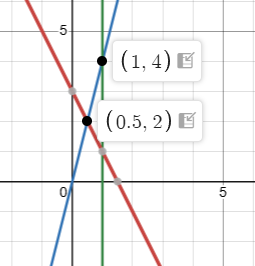
\includegraphics{3.5.1.png}\\
        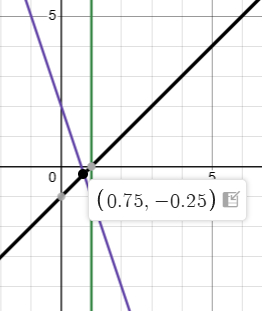
\includegraphics{3.5.2.png}

        note the first one image is player 1's payoffs and the second is p2's payoffs

        the red line represents going up and the blue line represents going down. the purple line represents left and the black, right.

        \item ~\\
        
        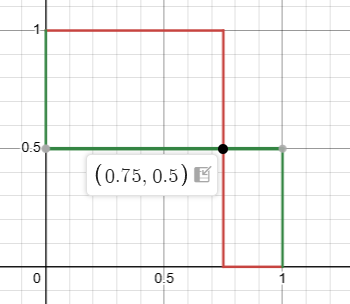
\includegraphics{3.5.3.png}
        
        the x axis represents \(x\), the probability of going up, and the y axis represents the probability of going Left. there are three NE. pure down left, pure up right, and the mix option shown by p1 75 25 between up and down, and p2 going 50 50 between left and right. \(x=.75,y=.5\)

    \end{itemize}
\end{enumerate}


% % remove strictly dominated pure strategies. 


% let the remaining options for player one be the set \(A\) and the set for player two to be \(B\). loop over the powerset of \(P=(\mathcal{P}(A)\setminus\emptyset\times \mathcal{P}(B)\setminus\emptyset)\). wlog let \(i\in P\)

% \(i[a]\) represents the support for which the iteration in the loop tries strategies for p1, and \(i[b]\) represents the strategies for p2.

% evaluate for mixed strategies by setting probabilities \(a_i\) for each option in \(i[a]\) and \(b_i\) in \(i[b]\). consider the set of equations over \(m\)
% \begin{equation}\label{3.1}
%     \sum_{n\in i[x_{-1}]} (x_{-1})_{n}\cdot f_x(n,m)
% \end{equation}
% where \(x\) denotes player 1 or 2 (stands in for \(a\) and \(b\)), \(x_{-1}\) represents the other player, and \(f_x(n,m)\)  represents the payoff for player \(x\) given player \(x\) does action \(m\) and player \(x_{-1}\) does action \(n\). 

% setting the set of equations over m of eq~\ref{3.1} equal and solving for \((x_{-1})_n\) results in either
% \begin{itemize}
%     \item a consistent set of equations
%     \item an inconsistent set of equations
% \end{itemize}

% if a consistent set of equations is found for both players, check if switching to any other pure strategy not in \(A\setminus i[x]\) is unilaterally better, for both players. if not, then a NE is found. otherwise, continue with a new element in the powerset \(P\)



\newpage
\section{4}

\begin{enumerate}
    \item if 1 person taking the bus generates enough shame to make the other 5 take the bus, then any additional bus takers also results in the plane takers switching. thus we need to find \(S\) such that
    
    \begin{equation}
        -S\cdot5< -1
    \end{equation}
    
    note that \(\frac{1}{5}\leq \frac{6-n}{n},n\in\{1,2,3,4\}\)
    
    we find that if \(S>1/5\), then everyone takes the bus. 

    % \item if \(S= 5+\varepsilon\), we see that the shame generated for a person taking the plane is \begin{equation}
    %     -(5+\varepsilon)\frac{6-N}{N}
    % \end{equation}

    % if everyone takes the plane, for \(\varepsilon>0\), deviating from taking the plane 


    \item for any value \(S>0\), there always exists a NE where everyone takes the plane, since no shame is generated, everyone gets 0 utility which is better than -1.

    \item when \(S=\frac{N}{8-N}\), there exists a NE where more than 1 person takes the bus and more than 1 person takes the plane. this is because the shame in taking the plane is equal to -1, thus they ahve no reason to deviate. 


    % \item yes. if \(S=5\), then for 1 person, it does not matter if they fly or take the bus since one person deviating results in the same payoff for flying as busing. 
    % \item yes. if \(S=5\), then at least for 1 person, it does not matter if they fly or take the bus since one person deviating results in the same payoff for flying as busing. 



\end{enumerate}


\end{document}